%╔════════════════════════════╗
%║	  Szablon dostosował	  ║
%║	mgr inż. Dawid Kotlarski  ║
%║		  16.10.2021		  ║
%╚════════════════════════════╝
\documentclass[12pt,twoside,a4paper,openany]{article}

    % ------------------------------------------------------------------------
% PAKIETY
% ------------------------------------------------------------------------

%różne pakiety matematyczne, warto przejrzeć dokumentację, muszą być powyżej ustawień językowych.
\usepackage{mathrsfs}   %Różne symbole matematyczne opisane w katalogu ~\doc\latex\comprehensive. Zamienia \mathcal{L} ze zwykłego L na L-transformatę.
\usepackage{eucal}      %Różne symbole matematyczne.
\usepackage{amssymb}    %Różne symbole matematyczne.
\usepackage{amsmath}    %Dodatkowe funkcje matematyczne, np. polecenie \dfac{}{} skladajace ulamek w trybie wystawionym (porównaj $\dfrac{1}{2}$, a $\frac{1}{2}$).

%język polski i klawiatura
\usepackage[polish]{babel}
%\usepackage{qtimes} % czcionka Times new Roman
\usepackage[OT4]{polski}
%\usepackage[cp1250]{inputenc}                       %Strona kodowa polskich znaków.

%obsługa pdf'a
\usepackage[pdftex,usenames,dvipsnames]{color}      %Obsługa kolorów. Opcje usenames i dvipsnames wprowadzają dodatkowe nazwy kolorow.
\usepackage[pdftex,pagebackref=false,draft=false,pdfpagelabels=false,colorlinks=true,urlcolor=blue,linkcolor=black,citecolor=green,pdfstartview=FitH,pdfstartpage=1,pdfpagemode=UseOutlines,bookmarks=true,bookmarksopen=true,bookmarksopenlevel=2,bookmarksnumbered=true,pdfauthor={Dawid Kotlarski},pdftitle={Praca Inznierska},pdfsubject={},pdfkeywords={transient recovery voltage trv},unicode=true]{hyperref}   %Opcja pagebackref=true dotyczy bibliografii: pokazuje w spisie literatury numery stron, na których odwołano się do danej pozycji.

%bibliografia
%\usepackage[numbers,sort&compress]{natbib}  %Porządkuje zawartość odnośników do literatury, np. [2-4,6]. Musi być pod pdf'em, a styl bibliogfafii musi mieć nazwę z dodatkiem 'nat', np. \bibliographystyle{unsrtnat} (w kolejności cytowania).
\usepackage[
backend=biber,
style=numeric,
sorting=none
]{biblatex}
\addbibresource{bibliografia.bib}
\usepackage{hypernat}                       %Potrzebna pakietowi natbib do wspolpracy z pakietem hyperref (wazna kolejnosc: 1. hyperref, 2. natbib, 3. hypernat).

%grafika i geometria strony
\usepackage{extsizes}           %Dostepne inne rozmiary czcionek, np. 14 w poleceniu: \documentclass[14pt]{article}.
\usepackage[final]{graphicx}
\usepackage[a4paper,left=3.5cm,right=2.5cm,top=2.5cm,bottom=2.5cm]{geometry}

%strona tytułowa
\usepackage{strona_tytulowa}

%inne
\usepackage[hide]{todo}                     %Wprowadza polecenie \todo{treść}. Opcje pakietu: hide/show. Polecenie \todos ma byc na koncu dokumentu, wszystkie \todo{} po \todos sa ignorowane.
\usepackage[basic,physics]{circ}            %Wprowadza środowisko circuit do rysowania obwodów elektrycznych. Musi byc poniżej pakietow językowych.
\usepackage[sf,bf,outermarks]{titlesec}     %Troszczy się o wygląd tytułów rozdziałów (section, subsection, ...). sf oznacza czcionkę sans serif (typu arial), bf -- bold. U mnie: oddzielna linia dla naglowku paragraph. Patrz tez: tocloft -- lepiej robi format spisu tresci.
\usepackage{tocloft}                        %Troszczy się o format spisu trsci.
\usepackage{expdlist}    %Zmienia definicję środowiska description, daje większe możliwości wpływu na wygląd listy.
\usepackage{flafter}     %Wprowadza parametr [tb] do polecenia \suppressfloats[t] (polecenie to powoduje nie umieszczanie rysunkow, tabel itp. na stronach, na ktorych jest to polecenie (np. moze byc to stroma z tytulem rozdzialu, ktory chcemy zeby byl u samej gory, a nie np. pod rysunkiem)).
\usepackage{array}       %Ładniej drukuje tabelki (np. daje wiecej miejsca w komorkach -- nie są tak ścieśnione, jak bez tego pakietu).
\usepackage{listings}    %Listingi programow.
\usepackage[format=hang,labelsep=period,labelfont={bf,small},textfont=small]{caption}   %Formatuje podpisy pod rysunkami i tabelami. Parametr 'hang' powoduje wcięcie kolejnych linii podpisu na szerokosc nazwy podpisu, np. 'Rysunek 1.'.
\usepackage{appendix}    %Troszczy się o załączniki.
\usepackage{floatflt}    %Troszczy się o oblewanie rysunkow tekstem.
\usepackage{here}        %Wprowadza dodtkowy parametr umiejscowienia rysunków, tabel, itp.: H (duże). Umiejscawia obiekty ruchome dokladnie tam gdzie są w kodzie źródłowym dokumentu.
\usepackage{makeidx}     %Troszczy się o indeks (skorowidz).

%nieużywane, ale potencjalnie przydatne
\usepackage{sectsty}           %Formatuje nagłówki, np. żeby były kolorowe -- polecenie: \allsectionsfont{\color{Blue}}.
%\usepackage{version}           %Wersje dokumentu.

%============
\usepackage{longtable}			%tabelka
%============


%PAGINA GÓRNA I DOLNA
\usepackage{fancyhdr}          %Dodaje naglowki jakie się chce.
\pagestyle{fancy}
\fancyhf{}
% numery stron w paginie dolnej na srodku
\fancyfoot[C]{\scriptsize DOKUMENTACJA PROJEKTU - PROGRAMOWANIE URZĄDZEŃ MOBILNYCH \\ 
\normalsize\sffamily  \thepage}


%\fancyhead[L]{\small\sffamily \nouppercase{\leftmark}}
\fancyhead[C]{\footnotesize \textit{PAŃSTWOWA WYŻSZA SZKOŁA ZAWODOWA W NOWYM SĄCZU}\\}

\renewcommand{\headrulewidth}{0.4pt}
\renewcommand{\footrulewidth}{0.4pt}

    % ------------------------------------------------------------------------
% USTAWIENIA
% ------------------------------------------------------------------------

% ------------------------------------------------------------------------
%   Kropki po numerach sekcji, podsekcji, itd.
%   Np. 1.2. Tytuł podrozdziału
% ------------------------------------------------------------------------
\makeatletter
    \def\numberline#1{\hb@xt@\@tempdima{#1.\hfil}}                      %kropki w spisie treści
    \renewcommand*\@seccntformat[1]{\csname the#1\endcsname.\enspace}   %kropki w treści dokumentu
\makeatother

% ------------------------------------------------------------------------
%   Numeracja równań, rysunków i tabel
%   Np.: (1.2), gdzie:
%   1 - numer sekcji, 2 - numer równania, rysunku, tabeli
%   Uwaga ogólna: o otoczeniu figure ma być najpierw \caption{}, potem \label{}, inaczej odnośnik nie działa!
% ------------------------------------------------------------------------
\makeatletter
    \@addtoreset{equation}{section} %resetuje licznik po rozpoczęciu nowej sekcji
    \renewcommand{\theequation}{{\thesection}.\@arabic\c@equation} %dodaje kropki

    \@addtoreset{figure}{section}
    \renewcommand{\thefigure}{{\thesection}.\@arabic\c@figure}

    \@addtoreset{table}{section}
    \renewcommand{\thetable}{{\thesection}.\@arabic\c@table}
\makeatother

% ------------------------------------------------------------------------
% Tablica
% ------------------------------------------------------------------------
\newenvironment{tabela}[3]
{
    \begin{table}[!htb]
    \centering
    \caption[#1]{#2}
    \vskip 9pt
    #3
}{
    \end{table}
}

% ------------------------------------------------------------------------
% Dostosowanie wyglądu pozycji listy \todos, np. zamiast 'p.' jest 'str.'
% ------------------------------------------------------------------------
\renewcommand{\todoitem}[2]{%
    \item \label{todo:\thetodo}%
    \ifx#1\todomark%
        \else\textbf{#1 }%
    \fi%
    (str.~\pageref{todopage:\thetodo})\ #2}
\renewcommand{\todoname}{Do zrobienia...}
\renewcommand{\todomark}{~uzupełnić}

% ------------------------------------------------------------------------
% Definicje
% ------------------------------------------------------------------------
\def\nonumsection#1{%
    \section*{#1}%
    \addcontentsline{toc}{section}{#1}%
    }
\def\nonumsubsection#1{%
    \subsection*{#1}%
    \addcontentsline{toc}{subsection}{#1}%
    }
\reversemarginpar %umieszcza notki po lewej stronie, czyli tam gdzie jest więcej miejsca
\def\notka#1{%
    \marginpar{\footnotesize{#1}}%
    }
\def\mathcal#1{%
    \mathscr{#1}%
    }
\newcommand{\atp}{ATP/EMTP} % Inaczej: \def\atp{ATP/EMTP}

% ------------------------------------------------------------------------
% Inne
% ------------------------------------------------------------------------
\frenchspacing                      
\hyphenation{ATP/-EMTP}             %dzielenie wyrazu w danym miejscu
\setlength{\parskip}{3pt}           %odstęp pomiędzy akapitami
\linespread{1.3}                    %odstęp pomiędzy liniami (interlinia)
\setcounter{tocdepth}{4}            %uwzględnianie w spisie treści czterech poziomów sekcji
\setcounter{secnumdepth}{4}         %numerowanie do czwartego poziomu sekcji 
\titleformat{\paragraph}[hang]      %wygląd nagłówków
{\normalfont\sffamily\bfseries}{\theparagraph}{1em}{}



    %polecenia zdefiniowane w pakiecie strona_tytulowa.sty
    \title{Zdrowy Spacer}
    \author{Kamil Pociecha}
    \authorI{Nicolas Świątnik}
    \authorII{}		%jeśli są dwie osoby w projekcie to zostawiamy:    \authorII{}
		
	\uczelnia{PAŃSTWOWA WYŻSZA SZKOŁA ZAWODOWA \\W NOWYM SĄCZU}
    \instytut{Instytut Techniczny}
    \kierunek{Informatyka Stosowana}
    \praca{DOKUMENTACJA PROJEKTOWA}
    \przedmiot{PROGRAMOWANIE URZĄDZEŃ MOBILNYCH}
    \prowadzacy{mgr inż. Dawid Kotlarski}
    \rok{2021}


%definicja składni mikrotik
\usepackage{fancyvrb}
\DefineVerbatimEnvironment{MT}{Verbatim}%
{commandchars=\+\[\],fontsize=\small,formatcom=\color{red},frame=lines,baselinestretch=1,} 
\let\mt\verb 
%zakonczenie definicji składni mikrotik

\usepackage{fancyhdr}    %biblioteka do nagłówka i stopki

			
\begin{document}
   
    \renewcommand{\figurename}{Rys.}    %musi byc pod \begin{document}, bo w~tym miejscu pakiet 'babel' narzuca swoje ustawienia
    \renewcommand{\tablename}{Tab.}     %j.w.
    \thispagestyle{empty}               %na tej stronie: brak numeru
    \stronatytulowa                     %strona tytułowa tworzona przez pakiet strona_tytulowa.tex
 
 \pagestyle{fancy}

    \newpage

    %formatowanie spisu treści i~nagłówków
    \renewcommand{\cftbeforesecskip}{8pt}
    \renewcommand{\cftsecafterpnum}{\vskip 8pt}
    \renewcommand{\cftparskip}{3pt}
    \renewcommand{\cfttoctitlefont}{\Large\bfseries\sffamily}
    \renewcommand{\cftsecfont}{\bfseries\sffamily}
    \renewcommand{\cftsubsecfont}{\sffamily}
    \renewcommand{\cftsubsubsecfont}{\sffamily}
    \renewcommand{\cftparafont}{\sffamily}
    %koniec formatowania spisu treści i nagłówków
     
    \tableofcontents    %spis treści
    \thispagestyle{fancy}
    \newpage

    
    \newpage

    
%%%%%%%%%%%%%%%%%%% treść główna dokumentu %%%%%%%%%%%%%%%%%%%%%%%%%

   	\newpage
\section{Ogólne określenie wymagań}		%1
%Ogólne określenie wymagań i zakresu programu (Czyli zleceniodawca określa wymagania programu)

Aplikacja ma się nazywać Zdrowy Spacer a jej grupą docelową mają być osoby aktywne fizycznie, które chcą kontrolować swoje wyniki.


\subsection{Podstawowe wymagania}  %1.1       

%większe wcięcie
\hspace{1cm} Aplikacja powinna ona spełniać podstawowe funkcjonalności takie jak: pomiary przebytych odległości, liczbę przebytych kroków, liczbę spalonych kalorii.%\footnote{Przykład odnośnika do książki\cite{legierski}.}.

\subsection{Dodatkowe wymagania}  %1.2       

%większe wcięcie
\hspace{1cm} Dodatkowo chcielibyśmy aby aplikacja rzutowała całą trasę na mapy, miała chociażby zapisywaną historię poprzednich tras do wglądu dla użytkownika, oczywiście umożliwiała ustalenie celu czy to podróży lub przebytych kroków/spalonych kalorii. Jako dodatkową funkcję przewidujemy też możliwość robienia zdjęć osiągniętego już celu, czyli np. zrobienie zdjęcia szczytu góry jako potwierdzenie osiągnięcia swojego celu. Chcielibyśmy również umożliwić naszym klientom logowanie się poprzez konta typu Facebook czy Google, co mogło by zautomatyzować proces logowania. Kolejną opcja którą przewidujemy by znalazła się w zamawianej przez nas aplikacji jest motyw typu jasny/ciemny dla uprzyjemnienia samego doświadczenia z korzystania z niej. Oczywiście aplikacja powinna mieć możliwość bezproblemowego działania w tle jak i również ewentualnego wykrycia ruchu bez jej inicjacji co przełoży się na to że sama zacznie rejestrować nasz spacer oraz aktywności.

%rysunek
%	\begin{figure}[!htb]
%	\begin{center}
%		
\includegraphics[width=2cm]{rys/logo.png}
%		\caption{Rysunek001}
%		\label{rys:rysunek001}
%	\end{center}
%\end{figure}

%Tutaj może coś być wpisane. \\Tutaj może coś być wpisane\footnote{Przykład odnośnika do strony www\cite{www1}.}. 

%tabelka
%\begin{tabela}
	%uwaga: w nawiasach [] nie może być odnośnika do literatury, jeżeli w dokumencie jest spis rysunków na początku, a spis literatury jest w kolejności cytowania (zmienia to numeracji)
%	{Tablica001}	%opis w spisie tabel
%	{Tablica001.}	%opis przy tabeli
%	{
%		\begin{tabular}{|c|c|} \hline
%			$U_n$ & $I_{zw}$ \\ \hline
%			$kV$  & $\%$      \\ \hline
%			7.2 & 100 \\ \hline
%		\end{tabular}
%	}
%	\label{tab:tablica001}
%\end{tabela}

%Tutaj może coś być wpisane. Tutaj może coś być wpisane. Tutaj może coś być wpisane.
   	\newpage
\section{Określenie wymagań szczegółowych}		%2
%Dokładne określenie wymagań aplikacji (cel, zakres, dane wejściowe) – np. opisać przyciski, czujniki, wygląd layautu, wyświetlenie okienek. Opisać zachowanie aplikacji – co po kliknięciu, zdarzenia automatyczne. Opisać możliwość dalszego rozwoju oprogramowania. Opisać zachowania aplikacji w niepożądanych sytuacjach.

\subsection{Opis wymagań}

\hspace{1cm}Aplikacja korzystać będzie z czujnika GPS, który umożliwi pomiar pokonanej odległości oraz rzutowanie trasy na mapę - w tym celu użyte zostaną mapy Google. Na podstawie przebytej odległości będzie można określić także liczbę kroków oraz ilość spalonych kalorii. Odległości przebyte w poprzednich dniach będą zapisywane w aplikacji co pozwoli użytkownikowi na porównywanie swoich wyników z poszczególnych dni. W przypadku osiągnięcia wyniku poniżej wybranej normy użytkownik zostanie powiadomiony o tym fakcie przez aplikację. 
W celu zmiany motywu aplikacji użyty zostanie czujnik światła, dzięki któremu w trakcie dnia będzie funkcjonował tryb ciemny a w nocy tryb jasny. 
Użytkownik będzie miał możliwość zaznaczenia na mapie swojego celu, do którego chce danego dnia dotrzeć. Następnie będzie miał możliwość by przy użyciu aparatu w telefonie wykonać zdjęcie osiągniętego miejsca docelowego. Zdjęcie to będzie zapisywanie w folderze aparatu a użytkownik będzie miał wgląd w zdjęcia swoich poprzednich celów.
Aby ułatwić proces logowania Użytkownik będzie miał możliwość logowania do aplikacji za pomocą Facebook’a lub konta Google.
Aplikacja będzie działała cały czas bez potrzeby inicjowania. Możliwe będzie jej działanie w tle a także zwijanie do paska.

\subsection{Layout aplikacji}

\hspace{1cm}Na stronie głównej aplikacja będzie wyświetlać przebytą odległość, liczbę wykonanych kroków oraz liczbę spalonych kalorii. W prawym górnym rogu znajduje się przycisk, który po jego naciśnięciu umożliwi zalogowanie się do aplikacji. W lewym górnym rogu znajduje się przycisk otwierający menu.
	\begin{figure}[!htb]
		\begin{center}
				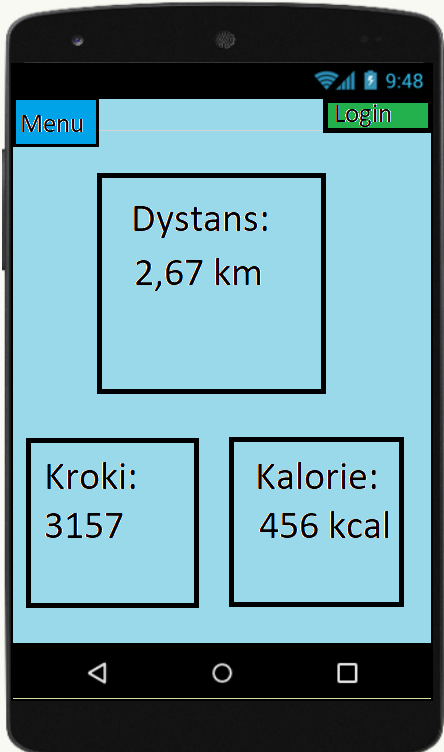
\includegraphics[width=3cm]{rys/Ap1.png}
				\caption{podstawowy layout aplikacji}
				\label{rys:rysunek001}
			\end{center}
	\end{figure}
\newline
Po otwarciu menu pojawi się lista w której znajdują się elementy takie jak: mapa - pokazuje przebytą trasę oraz umożliwia ustalenie swojego celu, wyniki - wyświetla wyniki osiągnięte w poprzednich dniach, Zdjęcia - otwiera galerię ze zdjęciami miejsc docelowych, wybierz normę - pozwala ustalić użytkownikowi jaki wynik chciałby osiągnąć.
\newline
  \begin{figure}[!htb]
	\begin{center}
		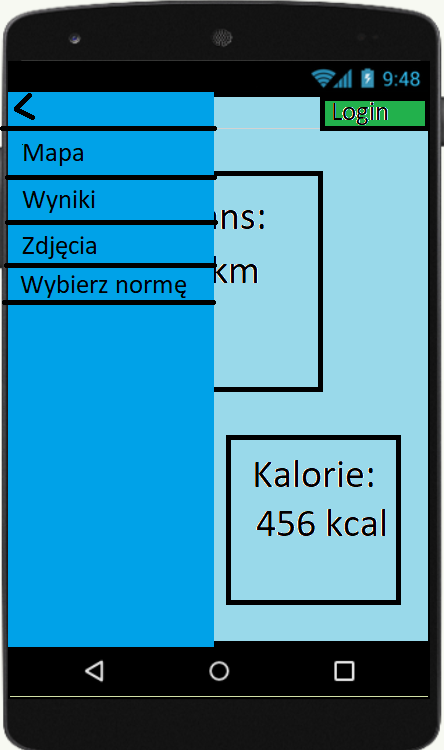
\includegraphics[width=3cm]{rys/Ap2.png}
		\caption{layout aplikacji po otwarciu menu}
		\label{rys:rysunek002}
	\end{center}
  \end{figure}







   	\newpage
\section{Projektowanie}		%3
%Opis przygotowania narzędzi (git, visual studio). Wybór i opis bibliotek, klas. Szkic layoutów. Pseudo kody. Opisy wykorzystanych algorytmów (np. algorytm sortowania). Dokładniejsze określenie założeń i działania aplikacji, (np.: ten przycisk otworzy takie okno a w tym oknie wpisujemy takie dane).

\subsection{Przygotowanie narzędzi Git oraz Visual Studio}

\hspace{1cm}W celu korzystania z narzędzia Git należy utworzyć na swoim komputerze repozytorium lokalne oraz dodać do niego pliki projektu. Na platformie GitHub utworzyć repozytorium zdalne, które umożliwi wszystkim autorom projektu współprace przy tworzeniu aplikacji.
\newline
W Visual Studio należy zainstalować dodatek opracowywanie aplikacji mobilnych za pomocą środowiska Xamarin oraz zestaw Android SDK, który umożliwia korzystanie z emulatora.
Do tworzenia projeku wybraliśmy szablo aplikacji mobilnej Xamarin.Forms.

\subsection{Biblioteki i klasy}
\hspace{1cm} \textbf{Biblioteka Xamarin.Essentials} udostępnia międzyplatformowy interfejs programowania aplikacji mobilnych (API). Jest ona dostępna jako pakiet NuGet i jest uwzględniana w każdym nowym projekcie w programie Visual Studio.
Biblioteka ta oferuje klasy, które zostaną przez nas użyte podczas tworzenia projektu.
\newline
\textbf{Geolokalizacja:}
\newline
\textbf{Klasa Geolocation} udostępnia interfejsy API do pobierania bieżących współrzędnych geolokalizacji urządzenia.
\newline
\textbf{Motyw aplikacji:}
\newline
Interfejs API RequestedTheme jest częścią klasy AppInfo i zawiera informacje dotyczące tematu żądanego dla uruchomionej aplikacji przez system.
\newline
\textbf{Akcelerometr:}
\newline
\textbf{Klasa Accelerometer} umożliwia monitorowanie czujnika przyspieszeniomierza urządzenia, który wskazuje przyspieszenie urządzenia w trójwymiarowej przestrzeni.
\newline
\textbf{GoogleMap:}
\newline
Firma Google oferuje natywny interfejs API mapowania dla systemu Android. Pozwala on na zmienianie punktu widzenia mapy, dodawanie i dostosowywanie znaczników, oznaczanie mapy za pomocą nakładek.
\newline
Wymagania wstępne Mapy API usługi Google: uzyskanie klucza Mapy API, zainstalowanie pakietu Xamarin.GooglePlayServices i Mapy pakietu z NuGet, określenie wymaganych uprawnień.
\newline
\textbf{Klasa GoogleMap} poprzez aplikację platformy Xamarin.Android będzie współdziałała z aplikacją Google Maps.
\newline
\newline
\textbf{Biblioteka Microsoft Authentication Library (MSAL)} pozwala na dodawanie uwierzytelniania do aplikacja. Umożliwi to logowanie do aplikacji przy użyciu Google lub Facebook.
\newline
\textbf{Klasa WebAuthenticator} umożliwia inicjowanie przepływów opartych na przeglądarce, które nasłuchują wywołania zwrotnego do określonego adresu URL zarejestrowanego w aplikacji.
\newline

\subsection{Layouty dla opcji z menu}
Po wybraniu z menu opcji \textbf{Mapa} na ekranie wyświetli się mapa pokazująca przebytą trasę oraz zaznaczająca miejsce w którym użytkownik w danym momencie się znajduje.
Na mapie będą się także wyświetlały zdjęcia miejsc docelowych zrobione przez użytkownika.
\begin{figure}[!htb]
	\begin{center}
		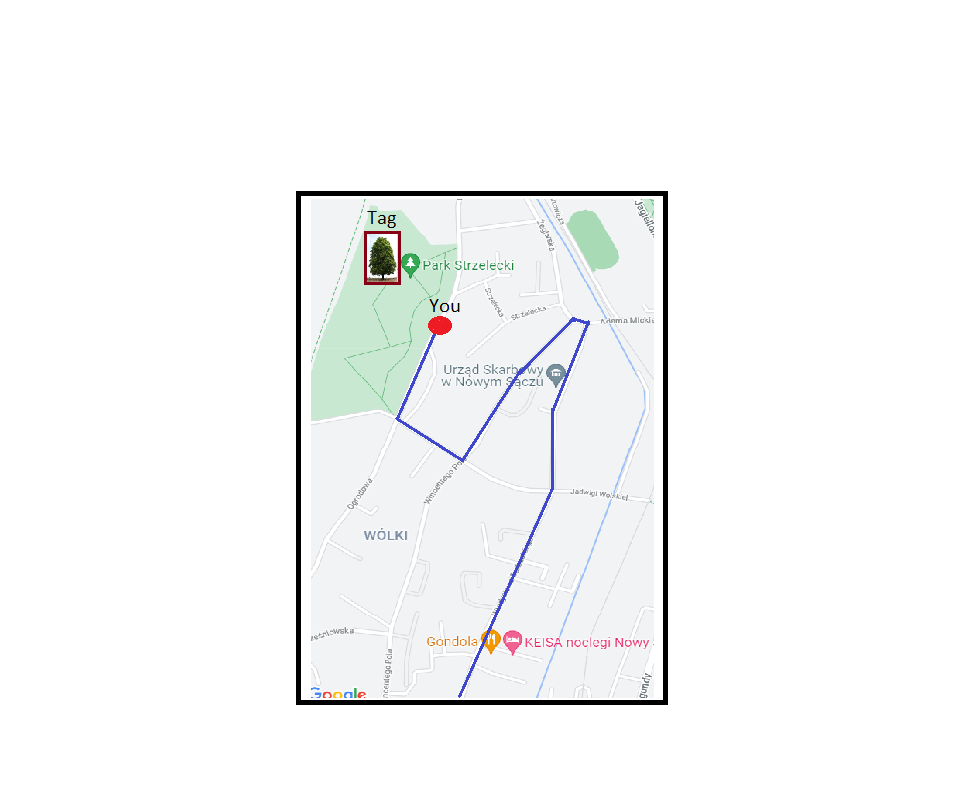
\includegraphics[width=16cm]{rys/Mapa.png}
		\caption{Layout - Mapa}
		\label{rys:rysunek003}
	\end{center}
\end{figure}
\newline Opcja \textbf{Wyniki} wyświetli stronę zawierającą wyniki z ostatnich 7 dni oraz najlepszy wynik z całej historii. Wśród wyświetlanych wyników znajdą się: Przybyta odległość, liczba kroków oraz liczba spalonych kalorii. Pozwoli to użytkownikowi na porównywanie swoich wyników oraz zmotywuje do poprawiania rekordowych wyników.
\begin{figure}[!htb]
	\begin{center}
		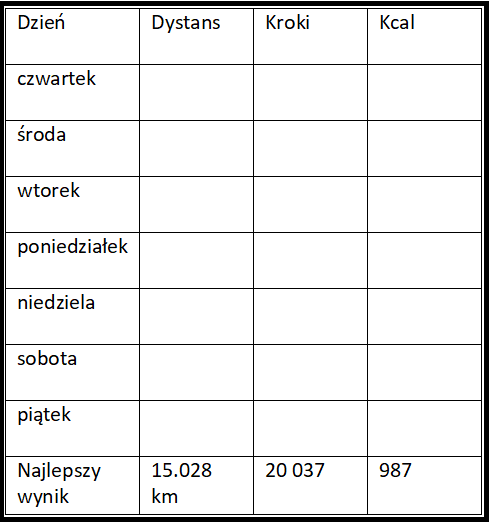
\includegraphics[width=8cm]{rys/Wyniki.png}
		\caption{Layout - Wyniki}
		\label{rys:rysunek004}
	\end{center}
\end{figure}
\newline Wybór opcji \textbf{Zdjęcia} otworzy galerie zdjęć wykonanych przez użytkownika. Zdjęcia będą przedstawiać miejsca docelowe uwiecznione aparatem telefonu.
\begin{figure}[!htb]
	\begin{center}
		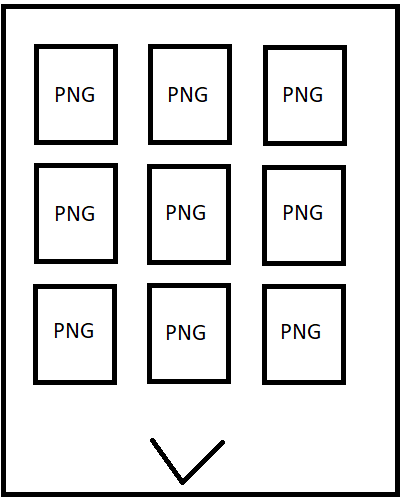
\includegraphics[width=6cm]{rys/Zdjęcia.png}
		\caption{Layout - Zdjęcia}
		\label{rys:rysunek005}
	\end{center}
\end{figure}
\newline
\newline Opcja \textbf{Wybierz} normę pozwala na wybranie dystansu jaki użytkownik planuje przebyć w ciągu dnia. Polega to na zaznaczeniu checkboxa obok wybranej odległości.
\begin{figure}[!htb]
	\begin{center}
		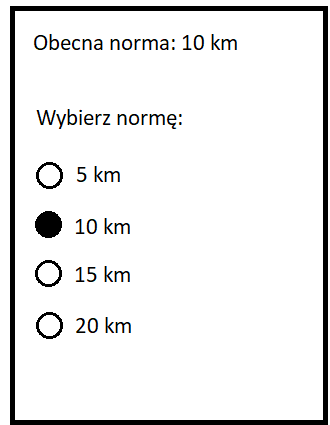
\includegraphics[width=8cm]{rys/Wybierz.png}
		\caption{Layout - Wybierz normę}
		\label{rys:rysunek006}
	\end{center}
\end{figure}
 
 
   	\newpage
\section{Implementacja}		%4
%Wkleić szkielet kodu, wraz z komentarzami. Opisać zmienne, struktury do czego służą. Opisać procedury, metody co wykonują. Opisać nowe zdefiniowane klasy. Opisać dziedziczenie. Opisać nowo utworzone pliki za co odpowiadają.
\textbf{Tworznie Menu:} \newline
Do stworzenia menu użyty został \textbf{Xamarin.forms Shell}, który zmiejsza złożoność tworzenia aplikacji, oferując podstawowe funkcje. Obejmuje on wspólne środowisko użytkownika nawigacji, schematu nawigacji i zintegrowanej procedury obsługi wyszukiwania.
\newline
\newline
\textbf{Dodawanie strony do menu na przykładzie elementu wyniki:}
\newline
W pliku \textbf{MainPage.xaml}:
\newline
\newline
\begin{figure}[!htb]
	\begin{center}
		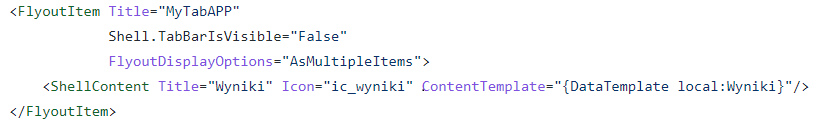
\includegraphics[width=12cm]{rys/item.png}
		\caption{Dodanie strony Menu do menu bocznego}
		\label{rys:rysunek007}
	\end{center}
\end{figure}
\newline
, gdzie \textbf{ic\_wyniki} to nazwa ikonki a \textbf{local:Wyniki} to odnośnik do plików strony "Wyniki", które znajdują się w folderze głównym projektu. 
\newline
\newline
\textbf{Dodawanie ikonek do projektu:} \newline
Ikonki pobrane zostały z \textbf{Android Asset Studio} w formacie ".png". \newline
Aby użyć ikonki w projekcie należy umieścić je w dwóch osobnych miejscach. Dla androida jest to folder \textbf{drawable} znajdujący się w folderze resources a dla systemu iOS folder \textbf{resources}.
\newline \newline
\newpage
Działanie menu bocznego w emulatorze Android 8.1:
\begin{figure}[!htb]
	\begin{center}
		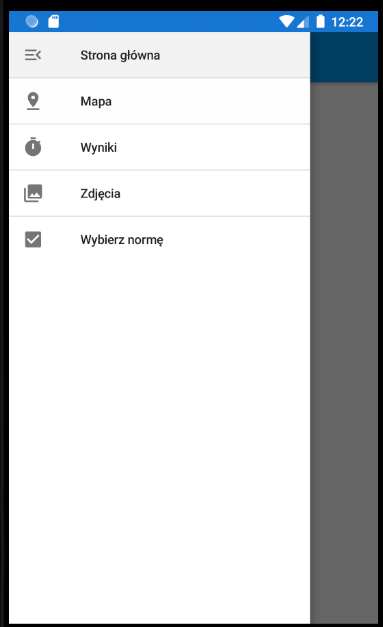
\includegraphics[width=6cm]{rys/ZSmenu.png}
		\caption{Widok menu bocznego}
		\label{rys:rysunek008}
	\end{center}
\end{figure}
\newline \newline
\begin{figure}[!htb]
	\begin{center}
		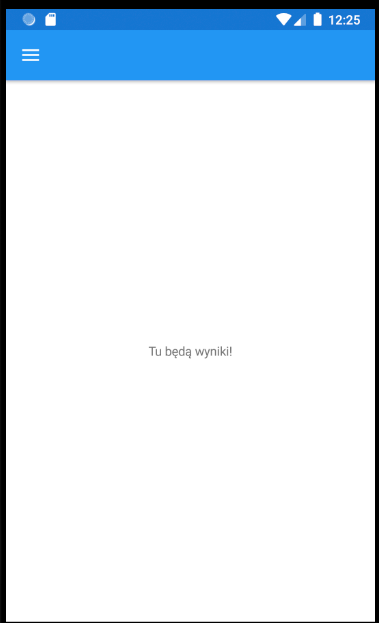
\includegraphics[width=5cm]{rys/ZSotwartastrona.png}
		\caption{Widok strony otwartej po wybraniu danej opcji z menu}
		\label{rys:rysunek009}
	\end{center}
\end{figure}
 \newline
 \textbf{Dodanie pól wyboru na stronie "Wybierz normę":} \newline
 Do stworzenia pól wyboru z których można wybrąć tylko jedną opcję potrzebne jest zainstalowanie pakietu Nuget \textbf{Xamarin.Forms.InputKit}. Przy użyciu tego pakietu można użyć opcji \textbf{RadioButton}, dzięki której tworzona jest lista z polami do wyboru. \newline \newline
 Fragment kodu z pliku \textbf{Wybierz\_norme.xml}: \newline
 \begin{figure}[!htb]
 	\begin{center}
 		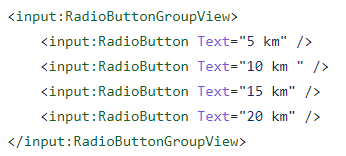
\includegraphics[width=12cm]{rys/checkboxy.png}
 		\caption{Dodanie opcji z polami do wyboru}
 		\label{rys:rysunek010}
 	\end{center}
 \end{figure}
  
  



   	\newpage
\section{Testowanie}	%5
%Opisujemy testy, sprawdzamy czy nie generuje błędów.



   	\newpage
\section{Podręcznik użytkownika}  %6
%Opis jak używać programu. Mogą być z zrzut ekranu razem z opisem. 


 
   
       
%%%%%%%%%%%%%%%%%%% koniec treść główna dokumentu %%%%%%%%%%%%%%%%%%%%%
		\newpage
    \addcontentsline{toc}{section}{Literatura}  
	\printbibliography


    \newpage

    \hypersetup{linkcolor=black}
    \renewcommand{\cftparskip}{3pt}
    \clearpage
    \renewcommand{\cftloftitlefont}{\Large\bfseries\sffamily}
    \listoffigures
    \addcontentsline{toc}{section}{Spis rysunków}
	\thispagestyle{fancy}
    \newpage
    \renewcommand{\cftlottitlefont}{\Large\bfseries\sffamily}
    \def\listtablename{Spis tabel}%
    \addcontentsline{toc}{section}{Spis tabel}\listoftables 
	\thispagestyle{fancy}
	


    %lista rzeczy do zrobienia: wypisuje na koñcu dokumentu, patrz: pakiet todo.sty
    \todos
    %koniec listy rzeczy do zrobienia
\end{document}
